\chapter{Machine Learning Models Explored}

This section describes the structure of each machine learning models used for various gamma-ray spectroscopy tasks. The simplest model explored is the DNN. Because of the high dimension of the input data, feature extraction methods will be implemented and compared. These methods include PCA, a DAE, and a CAE. 

The other general architecture that will be explored is a 1D CNN. 


\section{Dataset Used for the Hyperparameter Search}

In order to find optimal hyperparameters, a dataset is required. Because searching for optimal hyperparameters for each different dataset is infeasible due to computational cost, a simplified gamma-ray spectroscopy dataset will be used to optimize network hyperparameters. The dataset is comprised of unshielded gamma-ray spectra of ANSI isotopes simulated using GADRAS. A total of 125 spectra are simulated for each isotope. Each spectrum has parameters randomly selected from Table \ref{table:hyperparameter_dataset_parameters}. From this dataset, 25\% of samples are randomly chosen as the test dataset. Early stopping with a patience of 20 epochs is used to train each network. The maximum number of epochs was set to 200.

\begin{table}[H]
\centering
\caption{Range of parameters used for the hyperparameter search dataset.}
\label{table:hyperparameter_dataset_parameters}
\begin{tabular}{l|c|c|}
\cline{2-3}
 & \multicolumn{1}{r|}{Minimum} & \multicolumn{1}{l|}{Maximum} \\ \hline
\multicolumn{1}{|l|}{Integration Time {[}s{]}} & 60 & 3600 \\ \hline
\multicolumn{1}{|l|}{Linear Calibration Offset} & 0.8 & 1.2 \\ \hline
\multicolumn{1}{|l|}{Signal to Background Ratio} & 0.5 & 3.0 \\ \hline
\end{tabular}
\end{table}


\section{Hyperparameter Search Results}

The results of the hyperparameter searches are shown using a few random efficiency curves. These curves allow for reproducibility. These also allow for researchers who want to fit models to this dataset to have a performance benchmark. If you wanted to compare random hyperparameter search to more intelligent methods, you could compare using this.

\subsection{Dense Architecture}

Architecture and training hyperparamters are shown in Table \ref{table:hyperparameter_dataset_parameters}. Note, the number of nodes in each layers was made to decrease for each subsequent layer.

\begin{table}[H]
\centering
\caption{Range of hyperparameter explored for the DNN.}
\label{table:hyperparameter_dataset_parameters}
\begin{tabular}{l|c|c|c|}
\cline{2-4}
 & \multicolumn{1}{r|}{Minimum} & \multicolumn{1}{l|}{Maximum} & Sampling Method \\ \hline
\multicolumn{1}{|l|}{Number of Layers} & 1 & 3 & Uniform \\ \hline
\multicolumn{1}{|l|}{Nodes in Layer} & 10 & 1000 & Logarithmic \\ \hline
\multicolumn{1}{|l|}{Initial Learning Rate} & 10$^{-4}$ & 10$^{-1}$ & Logarithmic \\ \hline
\multicolumn{1}{|l|}{L2 Regularization Strength} & 10$^{-2}$ & 10$^{1}$ & Logarithmic \\ \hline
\multicolumn{1}{|l|}{Batch Size} & 16 & 512 & Power of Two \\ \hline
\multicolumn{1}{|l|}{Activation Function} & \multicolumn{2}{c|}{tanh, sigmoid, relu} & Uniform \\ \hline
\end{tabular}
\end{table}



Random efficiency curves for different reprocessing methods for the DNN are shown in Figure \ref{fig:random_efficiency_curve_DNN_preprocessing}. This figure implies that the optimum prepossessing step is BLANK. It's interesting that BLANK does better than BLANK. 

In addition to hyperparameters associated with the DNN's architecture and training, hyperparameters explored include the autoencoder used. Autoencoders can generate a different encoding based on a given architecture. The mean squared reconstruction error may not be the best metric to measure how good this encoding is as a preprocessing step. To determine an optimum preprocessing architecture for the dense and convolutional autoencoder, the choice of preprocessing architectures was added as a hyperparameter. The choices belong to the set with the N best reconstruction errors, respective of dense and convolution architecture.

\subsubsection{Hyperparameter Search Results - Autoencoders}

Now that we know optimized autoencoder architectures for the DNN, we need to optimize training hyperparameters. 

% https://machinelearningmastery.com/activation-regularization-for-reducing-generalization-error-in-deep-learning-neural-networks/

% \cite{Ranzato2007} Fig 6 shows you can freeze the unsupervised feature extraction network and update the classifier if you have enough data.

Sparse denoising autoencoders are included in in this work as feature extraction and dimension reduction techniques. Both autoencoders employ regularization techniques to ensure useful representations are learned. Both models includes $l1$ activity regularization as a method to induce sparsity on the networks activations, which increases generalization \cite{Goodfellow-et-al-2016}. 

Show how well autoencoders worked at spectrum reconstruction and background subtraction. See if there's a large difference between doing background subtraction and 



\begin{figure}[H]
	\centering
	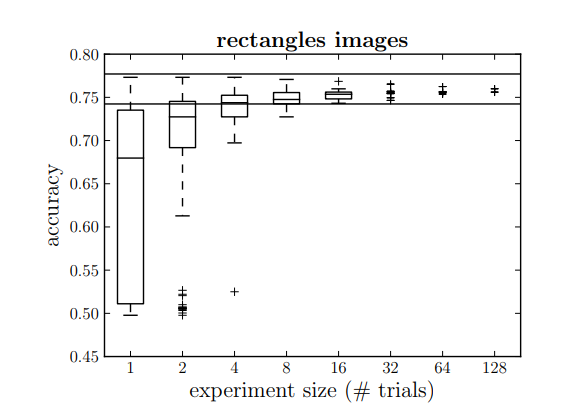
\includegraphics[width=0.8\linewidth]{model_choice_hyperparameter_search_images/Bergstra12_random_efficiency_curve}
	\caption{Random efficiency curves for the DAE. Sample curve from Bergstra 2012.}
	\label{fig:random_efficiency_curve_DAE}
\end{figure}


\begin{figure}[H]
	\centering
	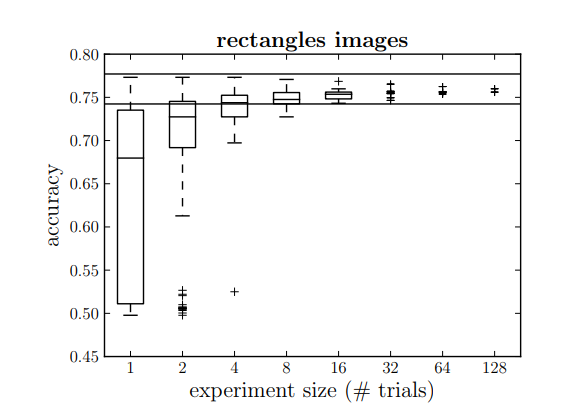
\includegraphics[width=0.8\linewidth]{model_choice_hyperparameter_search_images/Bergstra12_random_efficiency_curve}
	\caption{Random efficiency curves for the CAE. Sample curve from Bergstra 2012.}
	\label{fig:random_efficiency_curve_CAE}
\end{figure}

\subsubsection{Hyperparameter Search Results - Dense architecture with preprocessing }

\begin{figure}[H]
	\centering
	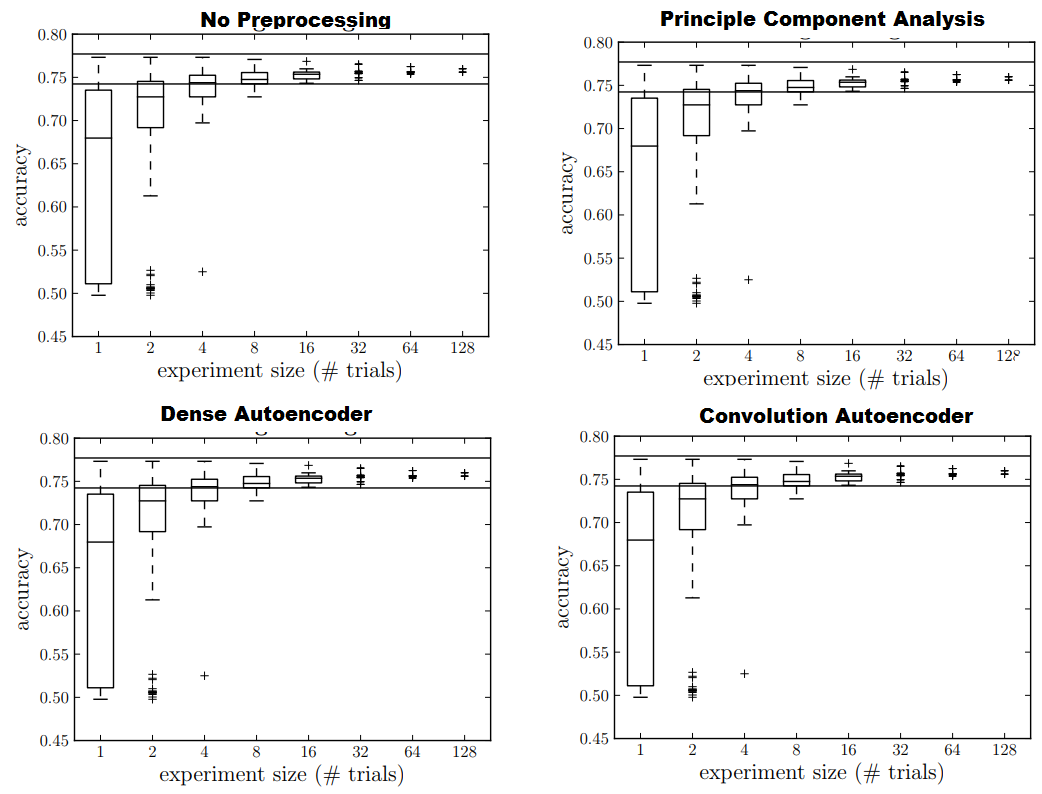
\includegraphics[width=0.99\linewidth]{model_choice_hyperparameter_search_images/Bergstra12_random_efficiency_curve_DNN}
	\caption{Random efficiency curves for the DNN with different fixed preprocessing steps. Sample curve from Bergstra 2012.}
	\label{fig:random_efficiency_curve_DNN_preprocessing}
\end{figure}

Because we know the optimum network using the preprocessing as fixed, we know optimum architectures for the autoencoders. We can now find, given all the autoencoder choices, which preprocessing technique should be better overall for the DNN. To do this we re-run the hyperparameter search with preprocessing included as a hyperparameter. These architectures and training hyperparameters will be used as the final  DNN model.

\begin{figure}[H]
	\centering
	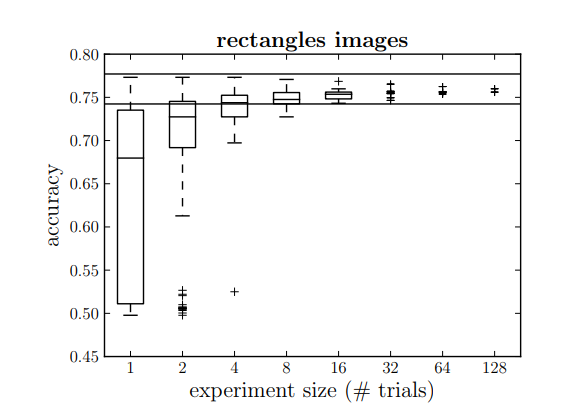
\includegraphics[width=0.8\linewidth]{model_choice_hyperparameter_search_images/Bergstra12_random_efficiency_curve}
	\caption{Random efficiency curves for the DNN with preprocessing steps as hyperparameters. Sample curve from Bergstra 2012.}
	\label{fig:random_efficiency_curve_DNN}
\end{figure}



\subsection{Convolution Architecture}

Just like the autoencoder, this can be done in one or two steps. One step: Train and optimize the entire network, convolution and dense layers. Two steps: Train and optimize the dense layer, using random initialization for non-trainable convolution filters. We'll probably go with the two-step.


\begin{figure}[H]
	\centering
	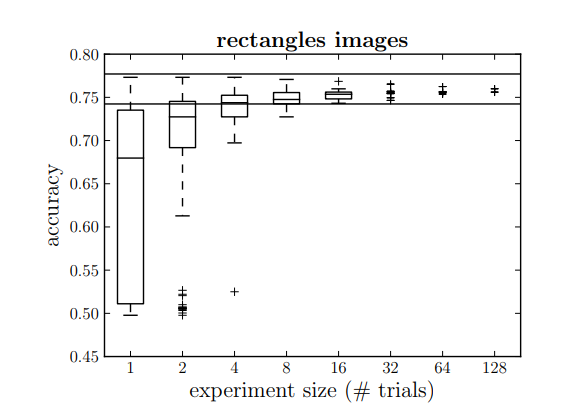
\includegraphics[width=0.8\linewidth]{model_choice_hyperparameter_search_images/Bergstra12_random_efficiency_curve}
	\caption{Random efficiency curves for the CNN, using non-trainable convolution filters. Sample curve from Bergstra 2012.}
	\label{fig:random_efficiency_curve_CAE}
\end{figure}




\begin{figure}[H]
	\centering
	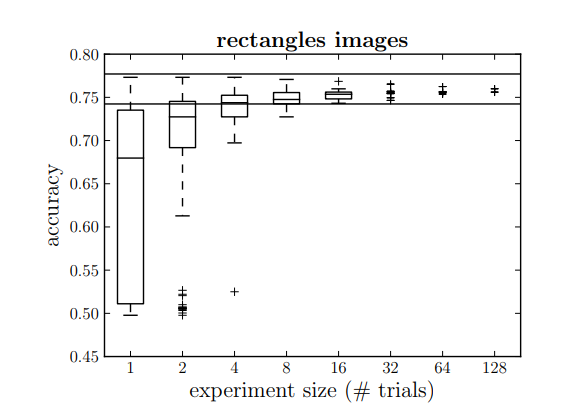
\includegraphics[width=0.8\linewidth]{model_choice_hyperparameter_search_images/Bergstra12_random_efficiency_curve}
	\caption{Random efficiency curves for the CNN with final convolution archetecture. Sample curve from Bergstra 2012.}
	\label{fig:random_efficiency_curve_CAE}
\end{figure}








\section{Summary of Final Model Architectures}

Learning curves are [definition, explanation]. Learning curves are used to determine a few things. We will use them to do [the following].

First, They are used as a sanity check, to make sure we are sampling our input space with enough granularity. To know we are sampling well enough, we should be sampling in a region where the curves are flat for both algorithms.

Secondly, Learning curves give us insight into which algorithm works better on the hyperparameter optimization dataset and simple version of the problem. We're expecting the CNN to outperform the DNN due to theoretical benefits of convolution architectures for our problem. We can also compare this curve to the final learning curves for the final datasets.



% Show learning curve to determine how many samples to add
\begin{figure}[H]
	\centering
	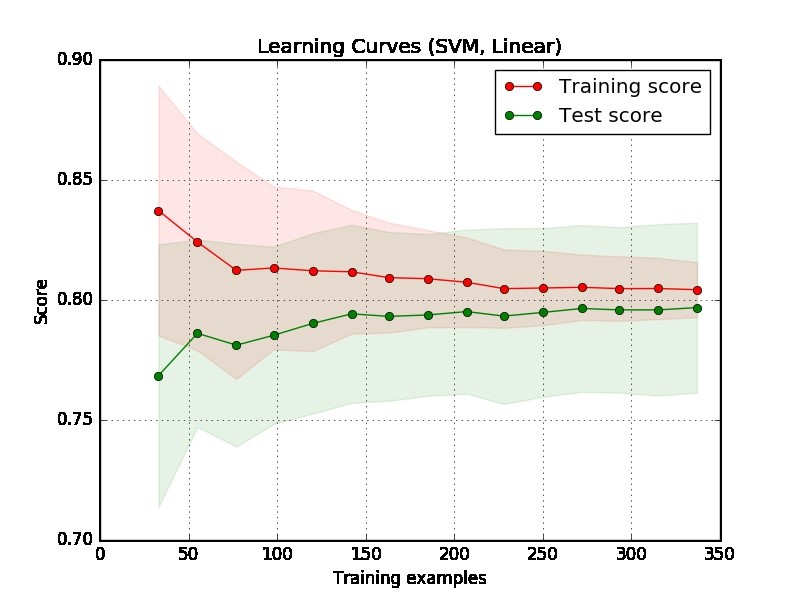
\includegraphics[width=0.8\linewidth]{model_choice_hyperparameter_search_images/learning_curve_dummy}
	\caption{Learning curves from the best DNN and CNN. X-axis will change to number of (input space sampling granularity? input space sampling divisions?). Shown: learning curve example.}
	\label{fig:Node}
\end{figure}








